\documentclass{article}

\usepackage{graphicx, titling}
\usepackage{float}
\usepackage[dutch]{babel}
\usepackage{hyperref}

\title{Human Pose Estimation Toepassing}
\author{Isaac Venus\\
Stan Vanhecke\\
Mathieu Vanooteghem}
\date{30/10/2020}

\begin{document}
\pagestyle{empty}


\begin{center}
	{{\Large Subfaculteit wetenschappen}
	
	\vspace{1cm}
	
	
\includegraphics[width=6cm]{2013-kulak-cmyk-highres.jpg}
	
	\vspace{1cm}
	
	\Large Probleemoplossen en ontwerpen 3}
	
	\vspace{2cm}

	{\Huge \textbf{Human Pose Estimation Toepassing}}
	
	\vspace{1cm}
	
	{\Large \textbf{Groepsnaam}}
	
	\vspace{1cm}
	
	{\Large \textbf{Isaac Venus}}\\
	{\Large \textbf{Stan Vanhecke}}\\
	{\Large \textbf{Mathieu Vanooteghem}}\\

\end{center}

\vspace{2cm}
{\Large Titularis : Koen Van Den Abeele}
\vspace{1cm}

{\Large Begeleider : Jens Goemaere}


\vspace{1cm}

\begin{center}
	{\Large Academiejaar 2020 - 2021}
\end{center}

\clearpage
\tableofcontents
\clearpage

\section*{Inleiding}
Aan materiaal in de medische wereld hangt steeds een stevig prijskaartje, daarom vroegen wij ons af of het niet mogelijk zou zijn om hulpmiddelen te ontwikkelen die heel budget vriendelijk zijn. Wat centraal staat is dat we hierbij geen gebruik maken van hoogtechnologische apparatuur en dat we ons beperken tot het gebruik van de camera's on onze laptops of gsm's. Het gaat dus meer om software dan het concreet bouwen van een apparaat. Hierbij richten wij ons op het gebied van 'Human Pose Estimation' (HPE), ook wel lichaamspositiebepaling. Dit is een techniek die aan de hand van neurale netwerken en deep learning de positie van personen schat op een foto.

\section{HPE, revolutionair?}
\subsection*{Inleiding}
Een (artificieel) neuraal netwerk of ANN is een netwerk geïnspireerd op een biologisch neuraal netwerk zoals die voorkomt in hersenen met de bedoeling om deze iets te doen leren. Het ANN is opgebouwd uit artificiële neuronen die een neuron in een brein moeten voorstellen. Al de neuronen zijn verbonden met andere neuronen en kunnen signalen uitsturen en ontvangen. In een ANN zijn de signalen getallen en kan elk neuron een bepaalde bewerking uitvoeren op een binnenkomend signaal voor deze verder te sturen. Elke connectie heeft ook een gewicht die bepaald hoe sterk het signaal is dat hij uitstuurt. Dit gewicht past zich aan als het neuraal netwerk leert. 

\subsection{Opbouw van een neuraal netwerk}
\subsubsection{Neuronen}
Zoals er in de inleiding staat is een artificieel neuron geïnspireerd op een neuron uit een brein. Elk neuron heeft een of meerdere inputs en één output die kan verzonden worden naar meerdere andere neuronen. De input van een neuron kan ofwel komen van de data die in het neuraal netwerk wordt gestoken of van andere neuronen. De output van de “output neurons” is hetgeen dat uit het programma komt. Om de output van een neuron te berekenen neem je de gewogen som van de inputs, met als gewicht de waarden van de connecties. Er wordt ook nog een bias opgeteld bij de output.

\subsubsection{Connecties}
Om te kunnen leren moet de data natuurlijk kunnen worden doorgegeven van het ene neuron naar de andere. Dit verloopt via een “connectie” die een bepaald gewicht heeft dat de sterkte en daarmee ook het belang van een bepaalde connectie weergeeft.

\subsubsection{Lagen}
Een neuraal netwerk bestaat uit meerdere lagen van neuronen, meer bepaald de input layer, hidden layers en output layer \ref{netwerk}. Zoals de namen wel duidelijk maken geef je de data aan de input layer en komen de berekende waarden uit de ouput layer. Daartussen zijn er eventueel hidden layers. Tussen twee lagen zijn er meerdere manieren van connecties tussen de neuronen mogelijk.

\begin{figure}
	\begin{center}
		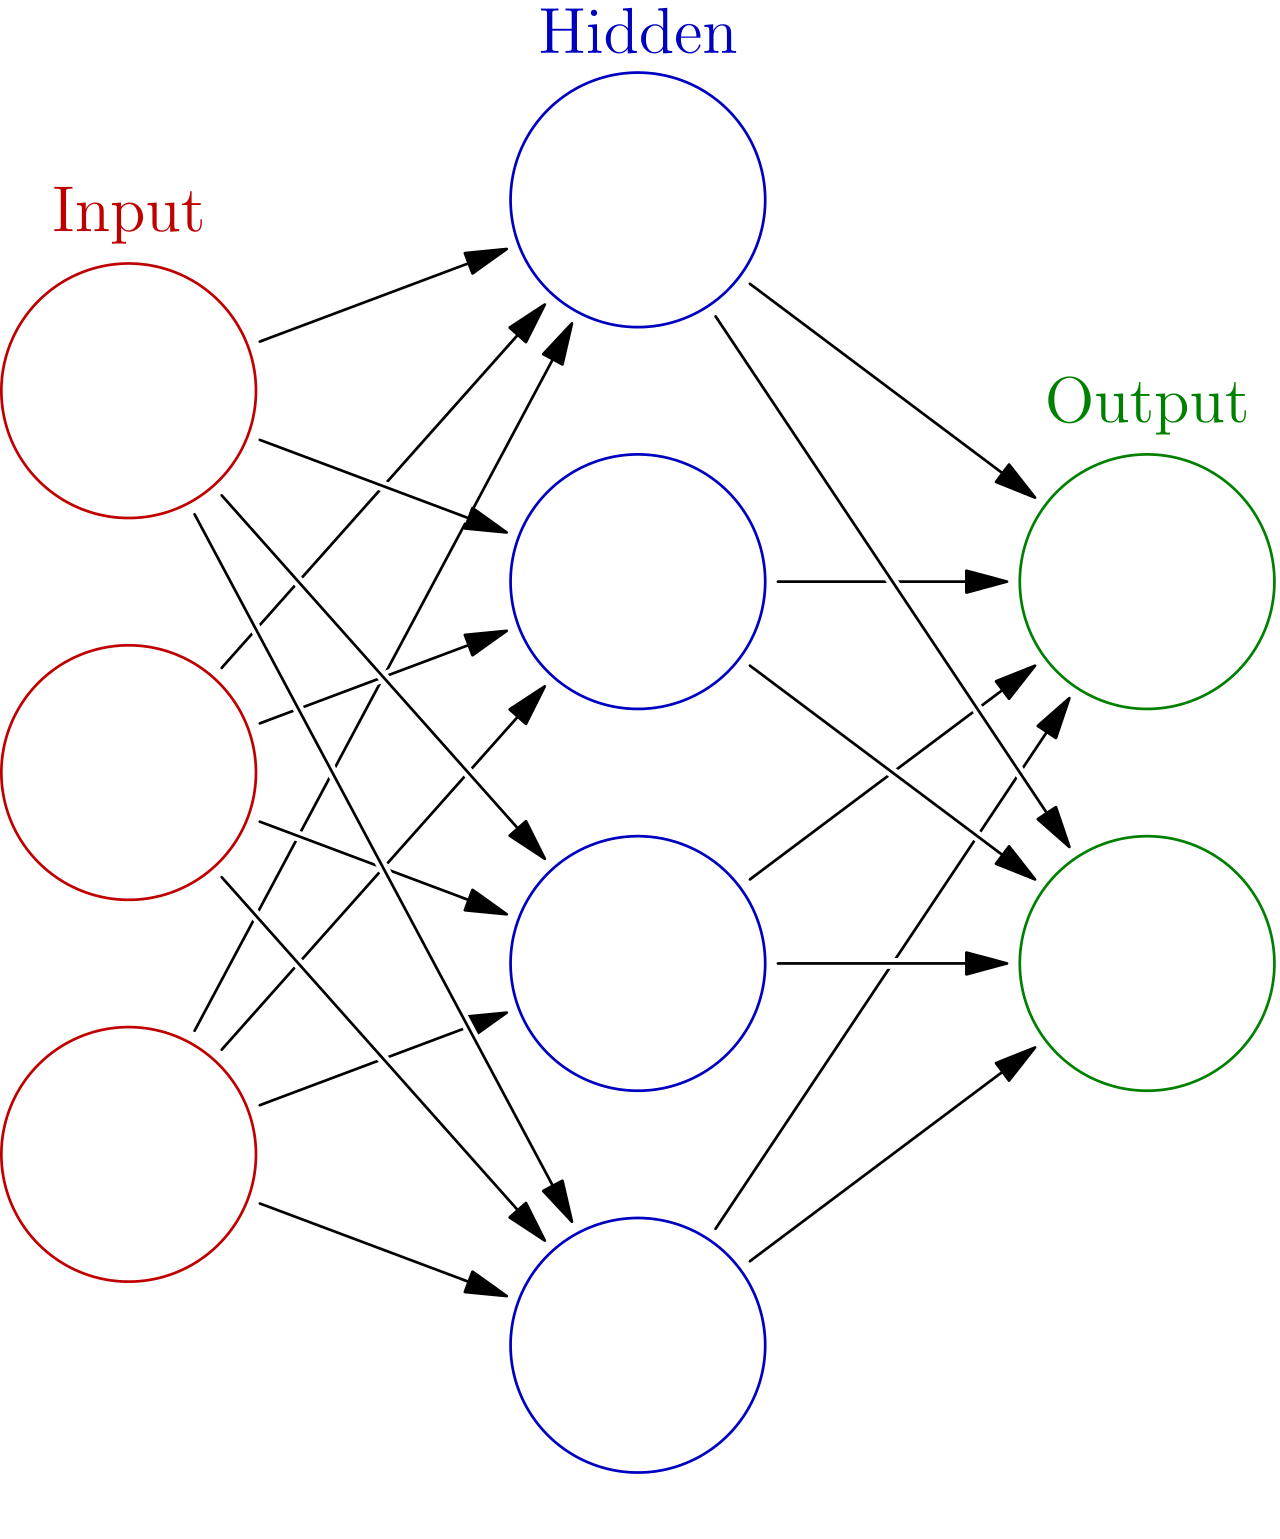
\includegraphics[width=8cm]{netwerk.png}
	\end{center}
	\caption{Voorbeeld van een neuraal netwerk. (afbeelding van wikipedia.org)}
	\label{netwerk}
\end{figure}

\subsection{Trainen van een neuraal netwerk}
Bij het programmeren van een neuraal netwerk weet je natuurlijk niet wat de gewichten zijn van alle connecties. Je moet het model dus doen leren. Dit doe je door de gewichten (over meerdere leercycli) aan te passen zodat de output zo goed mogelijk past bij het gewenste resultaat. Er zal altijd een bepaalde fout op de output zitten dus het model gaat nooit perfect zijn. Het trainen van een model is gedaan als de fout op de output niet meer verkleind en dus een minimum heeft bereikt. Het aanpassen van de gewichten gebeurt met een zekere learning rate. Dit bepaalt de grootte van de correcties die gebeuren bij de gewichten. Bij een grootte learning rate kan je model snel gedaan zijn met leren maar meer kans op een grotere fout op de output. Een kleine learning rate zal het trainen vertragen maar je uiteindelijke resultaat gaat beter zijn.



\section{Toepassingen}
Het doel is ergens in de paramedische wereld iets te vinden dat mogelijks gebruik kan maken van HPE, waardoor een goedkope oplossing kan worden ontwikkeld. Hierbij testen we dan mogelijke valkuilen en analyseren we of dit een goede en gemakkelijke oplossing zou zijn. We proberen dit dan allemaal op een methodische manier uit te werken, waarbij we een specifiek geval steeds breder gaan bekijken.

We zien een eerste toepassing in het opvolgen van de revalidatie na een schouderoperatie. Via een simpele foto gemaakt met de gsm kun je dan een week-na-week analyse uitvoeren van hoe de revalidatie evolueert. Een goedkope en degelijke oplossing.

Een tweede en uitgebreidere toepassing is het analyseren van de positie op de fiets. Veel amateurwielrenners hebben een slechte houding op de fiets en een professionele bikefitting kost al snel een paar honderd euro. Via HPE kunnen wij opnieuw met een simpele foto van de fietser in zijaanzicht tamelijk nauwkeurig de positie op de fiets gaan analyseren en eventuele correcties voorstellen. Opnieuw een goedkope oplossing die voor een breed publiek inzetbaar is. Voor professionele wielrenners zal HPE niet nauwkeurig genoeg zijn aangezien enkele millimeters daar soms het verschil maken tussen winnen en verliezen

\section{Toepassing 1: opvolgen van revalidatie na schouderoperatie}
	\subsection{Bepalen van de hoek tussen arm en lichaam}

We willen meten hoe ver een persoon zijn arm kan roteren met als doel om HPE toe te passen bij het opvolgen van de revalidatie na een schouderoperatie. Hiervoor willen we dus de hoek meten die een persoon kan maken tussen de arm en borst. Op figuur \ref{fig:skelet} komt dat dus neer op de hoek bepalen tussen de lijnstukken [32] en [21] voor de rechterarm en tussen [65] en [51] voor de linkerarm. Als we Openpose gebruiken om de positie te schatten van een persoon op een foto krijgen we als output de coördinaten van de verschillende knooppunten. Vanuit deze coördinaten kunnen we dan met behulp van de cosinusregel (\ref{eq:cos}) de gewenste hoek bepalen.

\begin{equation}
	cos(x,y) = \frac{x_1y_1+x_2y_2}{\sqrt{x_1^2+x_2^2} \sqrt{y_1^2+y_2^2}}
	\label{eq:cos}
\end{equation}

We kunnen de revalidatie opvolgen door verschillende bewegingen van de schouder te bestuderen. Bij een foto vanuit vooraanzicht kunnen we kijken hoe ver de patiënt zijn arm zijwaarts omhoog kan brengen. Bij een foto genomen vanuit zijaanzicht kunnen we meten hoe ver hij de arm vooruit kan omhoog steken. Belangrijk is wel dat de foto's zo goed mogelijk vanuit een bepaald aanzicht te nemen aangezien HPE in 2D werkt. Als de foto scheef genomen wordt, heeft het meten van de hoeken niet veel zin.

Week na week kan dan bijvoorbeeld een foto van de patiënt in dezelfde positie geanalyseerd worden om zo de voortgang van de revalidatie objectief te kunnen beoordelen. 

\begin{figure}[H]
	\centering
	\caption{Voorstelling van de positie bepaald via Openpose}
	\label{fig:skelet}
	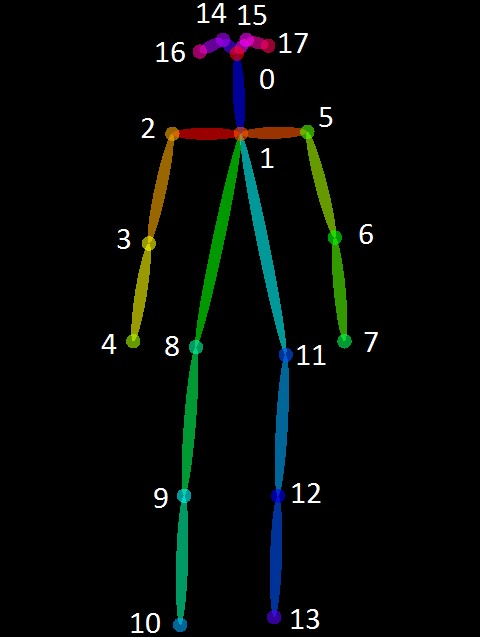
\includegraphics[width=.5\textwidth]{HPE_skelet}
\end{figure}


	\subsection{Voorlopige resultaten}
\subsubsection*{Inleiding}
Via openpose krijgen we de coördinaten van alle punten die openpose kan herkennen. Hiermee kunnen we dan verder onderzoek doen. Voor het moment zijn we in staat om hoeken tussen bepaalde lichaamsdelen te berkenen met als doel objectieve gegevens te bekomen tijdens bijvoorbeeld een revalidatie na een ongeval.
\subsubsection{Wiskundige achtergrond}
Om de hoek tussen twee lichaamsdelen te berekenen gebruiken we de cosinusregel. Hier volgt een klein beetje duiding over hoe we die precies gebruiken. Een verduidelijkende figuur is \ref{cos}.\\
\begin{figure}
	\begin{center}
		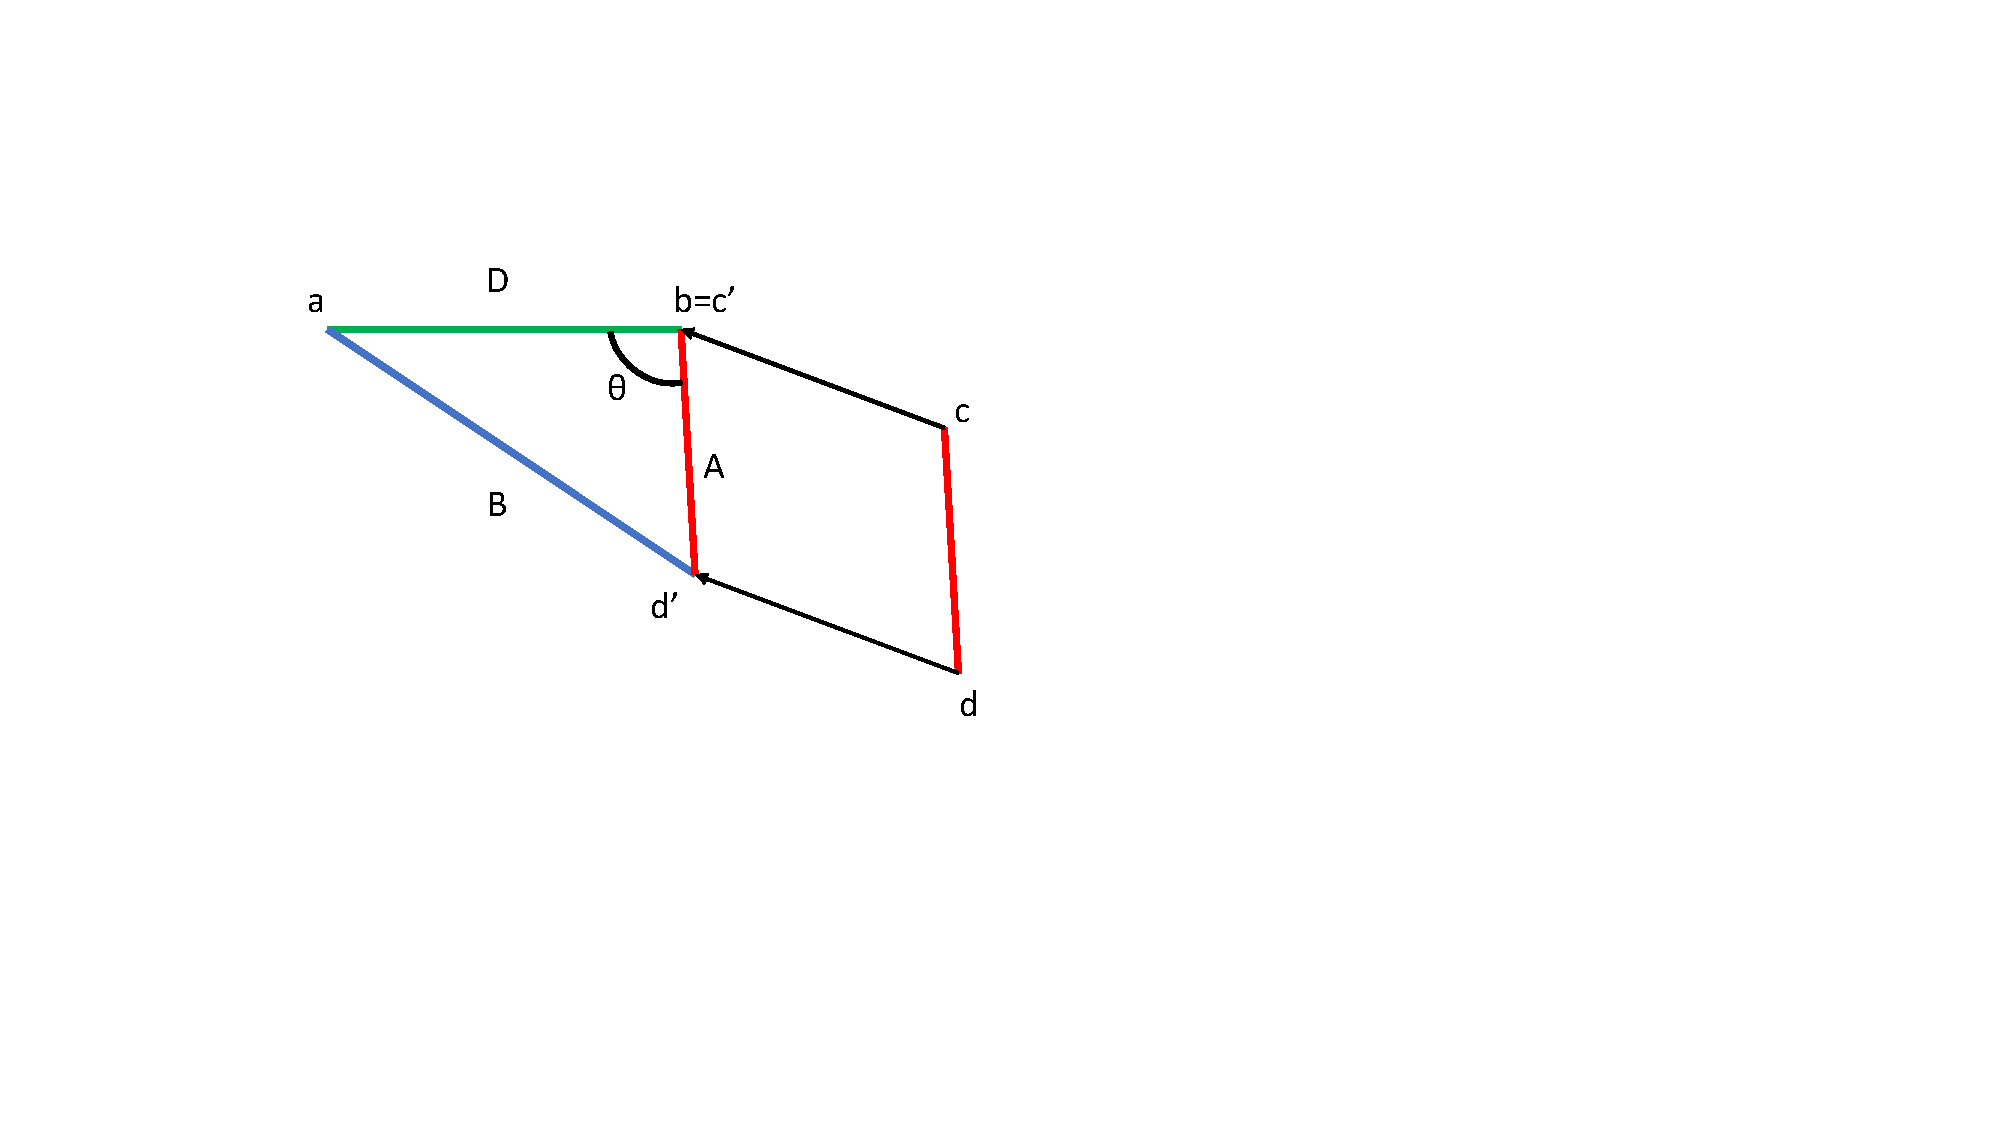
\includegraphics[width=10cm]{cos.pdf}
	\end{center}
	\caption{Hoek tussen 2 lichaamsdelen}
	\label{cos}
\end{figure}
We stellen \(a, b\) de coördinaten die het eerste lichaamsdeel afbakenen en \(c, d\) de coördinaten van het tweede lichaamsdeel. De hoek tussen de lichaamsdelen is dan de \(\theta\) van op de figuur. We kunnen gewoon de cosinusregel gebruiken om de hoek te bepalen als we \(c\) op \(b\) leggen. We krijgen dan
\[B^2 = A^2 + D^2 -2\cdot A\cdot D\cos\theta\]
en dus
\[\cos\theta = \frac{A^2 + B^2 - B^2}{2\cdot A\cdot D}\]
met
\[A = \sqrt{(d_x - c_x)^2 + (d_y - c_y)^2}\]
\[B = \sqrt{(b_x - a_x + d_x - c_x)^2 + (b_y - a_y + d_y - c_y)^2}\]
\[D = \sqrt{(b_x - a_x)^2 + (b_y - a_y)^2}\]
Als we dus de 4 coördinaten weten kunnen we de hoek bepalen.
\subsubsection{Voorbeeld}
Een voorbeeld bij het bepalen van een hoek tussen is afbeelding \ref{samen}. Als we de hoek bereken tussen de ruggengraat (rood) en het opperarmbeen(licht oranje) krijgen we als waarde:
\begin{itemize}
	\item 1: 21.63 graden
	\item 2: 78.06 graden
	\item 3 130.00 graden
\end{itemize}
\begin{figure}
	\begin{center}
		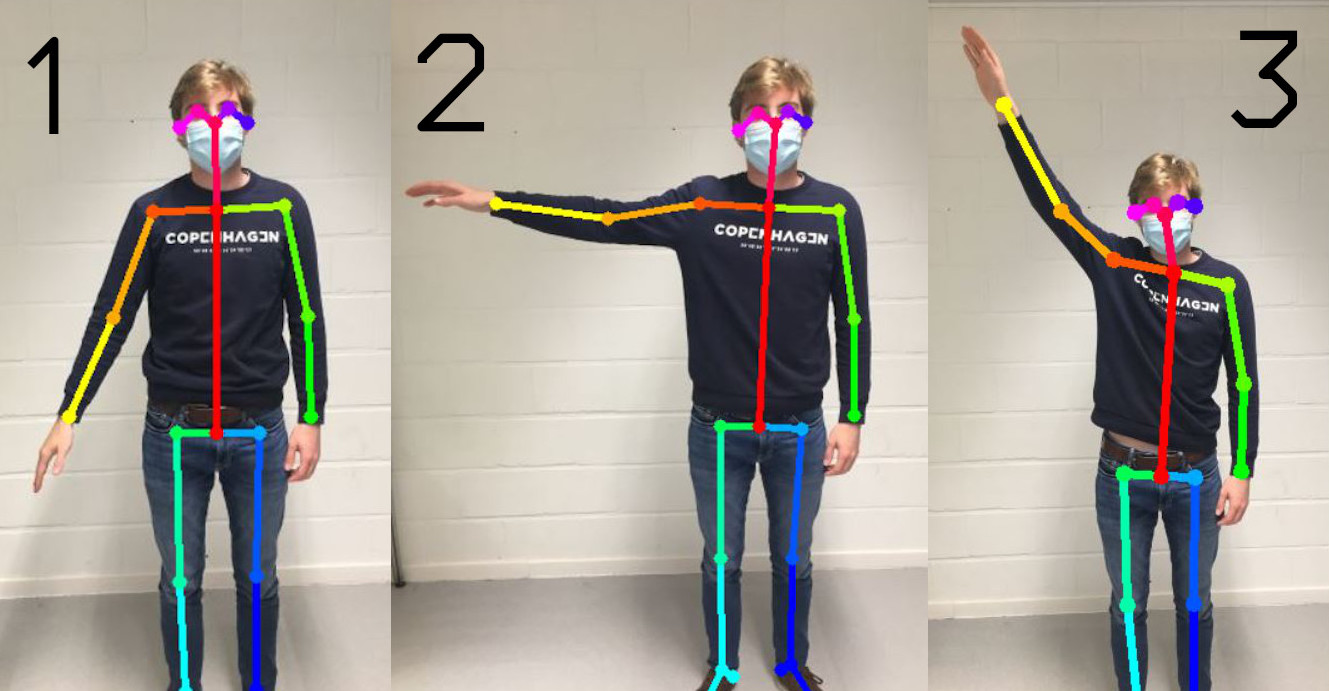
\includegraphics[width=12cm]{samen.jpg}
	\end{center}
	\caption{Voorbeeld bij het bepalen van een hoek.}
	\label{samen}
\end{figure}
	\subsection{Voorlopige conclusies}

\section{Toepassing 2: fietspositie bepalen}

\section{Vakintegratie}
Het is natuurlijk belangrijk om dit project een plaats te geven binnen onze opleiding ingenieurswetenschappen. We bekijken welke vakken uit de eerste 3 semesters van onze bachelor het meest gebruikt worden tijdens dit project. De belangrijkste link is met het vak Begingselen van programmeren. In dit vak leerden we werken met Python en verworven we inzicht in het programmeren. Wat heel handig is, want tijdens ons project maken we veelvuldig gebruik van Python. Elk zelf gemaakt programma is geschreven in Python en ook Openpose maak gebruik van deze computertaal. Verder maakt wiskunde ook een groot deel uit van ons project, want het berekenen van hoeken of afstanden kan niet zonder de wiskunde. We gebruiken hierbij kennis uit verschillende wiskundige vakken zoals, Analyse \& calclus en Lineaire algebra. Als laatste kunnen we Statistiek ook nog linken aan dit project aangezien Openpose enkel een schatting geeft van de lichaamspositie. Het werkt met \textit{heatmaps} en kiest per knooppunt dan het coördinaat met de hoogste kans. We gebruiken zelf geen statistische technieken, maar de kennis die we verworven hebben in dit vak helpt ons wel bij het begrijpen van Openpose. 

Met vakken die te maken hebben met energie en materie, zoals Algemene natuurkunde deel 1,2,3 is er geen link. Dit zou wel mogelijk zijn als je Openpose met videomateriaal gebruikt. Dan zou je de snelheden van knooppunten kunnen berekenen. Bijvoorbeeld bij de worp van een bal de snelheid van de hand berekenen. Maar dit is niet wat wij doen in ons project.
\section{Planning}
(gantt chart enzo\texttt{})

\section{Referenties}


\end{document}